\documentclass[11pt,a4paper]{article}

\usepackage[margin=1in]{geometry}
\usepackage[T1]{fontenc}
\usepackage[utf8]{inputenc}
\usepackage{parskip}
\usepackage[activate={true,nocompatibility},protrusion=true,expansion=false]{microtype}
\usepackage{graphicx}
\usepackage{xcolor}
\usepackage{tcolorbox}
\usepackage{listings}
\usepackage{amsmath,amssymb}
\usepackage{enumitem}
\usepackage{booktabs}
\usepackage{tikz}
\usetikzlibrary{shapes.geometric, arrows.meta, positioning, calc}
\usepackage{titlesec}
\usepackage[hidelinks,bookmarks=true,bookmarksnumbered=true]{hyperref}

\sloppy
\emergencystretch=3em

% Colours
\definecolor{primary}{RGB}{30,100,180}
\definecolor{accent}{RGB}{30,140,80}
\definecolor{warn}{RGB}{220,130,20}
\definecolor{danger}{RGB}{190,40,50}
\definecolor{soft}{RGB}{240,240,245}
\definecolor{codebg}{RGB}{248,249,252}

\hypersetup{linkcolor=primary, urlcolor=primary, citecolor=primary}

\titleformat{\section}{\LARGE\bfseries\color{primary}}{\thesection.}{0.6em}{}
\titleformat{\subsection}{\Large\bfseries\color{accent}}{\thesubsection}{0.5em}{}
\titleformat{\subsubsection}{\large\bfseries}{\thesubsubsection}{0.4em}{}
\titlespacing*{\section}{0pt}{16pt}{8pt}
\titlespacing*{\subsection}{0pt}{12pt}{4pt}

% Code listings in plain English style
\lstdefinestyle{plain}{
  basicstyle=\ttfamily\footnotesize,
  backgroundcolor=\color{codebg},
  breaklines=true,
  frame=single,
  rulecolor=\color{primary!40},
  keywordstyle=\color{primary}\bfseries,
  stringstyle=\color{accent},
  commentstyle=\color{gray}\itshape,
  language=Python,
  showstringspaces=false,
  xleftmargin=8pt, xrightmargin=8pt,
  framesep=4pt,
}
\lstset{style=plain}

% Boxes
\newtcolorbox{why}{colback=primary!5, colframe=primary!60!black, boxrule=0.5pt,
  arc=2pt, left=6pt, right=6pt, top=4pt, bottom=4pt,
  title={\textbf{Why it matters}}, fonttitle=\bfseries\color{white},
  colbacktitle=primary!80!black, attach title to upper}
\newtcolorbox{alt}{colback=warn!5, colframe=warn!60!black, boxrule=0.5pt,
  arc=2pt, left=6pt, right=6pt, top=4pt, bottom=4pt,
  title={\textbf{Alternatives we considered}}, fonttitle=\bfseries\color{white},
  colbacktitle=warn!80!black, attach title to upper}
\newtcolorbox{keyidea}{colback=accent!5, colframe=accent!60!black, boxrule=0.5pt,
  arc=2pt, left=6pt, right=6pt, top=4pt, bottom=4pt,
  title={\textbf{Plain-English summary}}, fonttitle=\bfseries\color{white},
  colbacktitle=accent!80!black, attach title to upper}

\title{\vspace{-1.5cm}\Huge\textbf{Customer Support Copilot}\\[8pt]
       \Large\textit{Beginner's Documentation Guide}\\[4pt]
       \normalsize A gentle walk-through of every part of the system, in simple language}
\author{Project Team}
\date{\today}

\begin{document}
\maketitle

\vspace{-20pt}
\begin{center}
\colorbox{soft}{\parbox{0.9\textwidth}{\small
\textbf{Who is this document for?}\\[2pt]
Anyone who wants to understand \emph{how} the Customer Support Copilot works and \emph{why} we built it the way we did --- without needing a machine-learning background. Each section starts with a plain-English summary, then adds the technical detail. If you only read the green boxes, you still understand the project.
}}
\end{center}

\tableofcontents
\clearpage

% ==================================================================
\section{Project Overview}

\subsection{The one-sentence pitch}

\begin{keyidea}
A chatbot that answers customer questions from a company's knowledge base, opens a support ticket when it does not know, and refuses to make up answers.
\end{keyidea}

\subsection{The problem we are solving}

Imagine a large company with thousands of policy documents (Social Security in our case). A customer asks a question. They want:

\begin{enumerate}[leftmargin=*, itemsep=2pt]
\item A direct, correct answer.
\item A reference to the exact policy section the answer came from (so they can verify).
\item If the system cannot find an answer, a \emph{ticket} that gets routed to a human --- not a guess.
\end{enumerate}

The way most chatbots fail is the third point. They almost never say ``I don't know''. They guess. A guess that sounds confident is more dangerous than no answer at all, because the customer trusts it.

\subsection{Our approach, in one picture}

Every user question goes through this pipeline:

\begin{center}
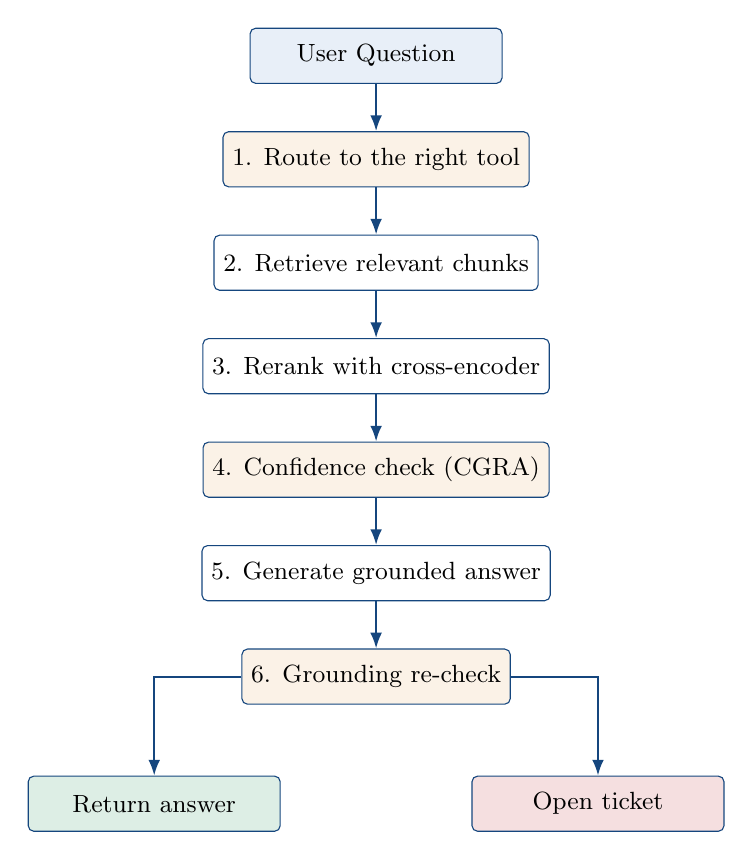
\begin{tikzpicture}[
  every node/.style={font=\small},
  b/.style={rectangle, rounded corners=2pt, draw=primary!70!black, fill=white,
             minimum width=32mm, minimum height=7mm, align=center},
  arr/.style={-{Latex[length=2mm]}, thick, draw=primary!70!black},
]
\node[b, fill=primary!10]                 (q)  {User Question};
\node[b, fill=warn!10,   below=6mm of q]  (rt) {1. Route to the right tool};
\node[b,                  below=6mm of rt] (rc) {2. Retrieve relevant chunks};
\node[b,                  below=6mm of rc] (rk) {3. Rerank with cross-encoder};
\node[b, fill=warn!10,    below=6mm of rk] (cg) {4. Confidence check (CGRA)};
\node[b,                  below=6mm of cg] (gn) {5. Generate grounded answer};
\node[b, fill=warn!10,    below=6mm of gn] (gr) {6. Grounding re-check};
\node[b, fill=accent!15,  below left=9mm and -5mm of gr] (an) {Return answer};
\node[b, fill=danger!15,  below right=9mm and -5mm of gr] (tk) {Open ticket};
\draw[arr] (q) -- (rt);
\draw[arr] (rt) -- (rc);
\draw[arr] (rc) -- (rk);
\draw[arr] (rk) -- (cg);
\draw[arr] (cg) -- (gn);
\draw[arr] (gn) -- (gr);
\draw[arr] (gr) -| (an);
\draw[arr] (gr) -| (tk);
\end{tikzpicture}
\end{center}

Six steps. Three of them are \emph{check} steps --- the orange boxes. The job of the check steps is to notice when the system is about to say something it cannot back up, and stop it.

\subsection{What this document will cover}

\begin{itemize}[leftmargin=*, itemsep=2pt]
\item \textbf{Section 2 (Workflow)} walks through the six steps in order.
\item \textbf{Section 3 (Why each component)} explains each piece: what it is, what it does, why it is there.
\item \textbf{Section 4 (Alternatives)} shows what else we could have used and why we picked what we picked.
\item \textbf{Section 5 (Code snippets)} shows the most important pieces of code with plain-English commentary.
\item \textbf{Section 6 (End-to-end story)} follows a single query all the way through the system.
\end{itemize}

\clearpage
% ==================================================================
\section{Workflow, Step by Step}
\label{sec:workflow}

\subsection{Step 1 --- Route to the right tool}

\begin{keyidea}
Different questions need different answers. ``What documents do I need to apply?'' needs to look things up in the knowledge base. ``I can't log in'' needs to open a support ticket. The router decides which one.
\end{keyidea}

The router reads the question and chooses one of three tools:

\begin{itemize}[leftmargin=*, itemsep=1pt]
\item \texttt{SearchKB} --- search the knowledge base for relevant passages
\item \texttt{GetPolicy} --- look up a specific policy section by id
\item \texttt{CreateTicket} --- escalate to a human
\end{itemize}

We offer two implementations:

\begin{enumerate}[leftmargin=*, itemsep=2pt]
\item \textbf{Keyword router} (default): fast rules. If the question contains ``login'', ``password'', ``broken'' $\rightarrow$ ticket. If it contains ``section'', ``policy'', ``rule'' $\rightarrow$ get-policy. Otherwise $\rightarrow$ search.
\item \textbf{Learned router} (optional): a small trained classifier. Reads the question as a 384-dimensional vector (via MiniLM), then picks the tool with a logistic-regression head. This catches paraphrases like ``stuck on the sign-in page'' which the keyword router would miss.
\end{enumerate}

\subsection{Step 2 --- Retrieve relevant chunks}

\begin{keyidea}
We have already split the knowledge base into thousands of short passages called ``chunks''. Given a question, find the top 20 chunks most likely to contain the answer.
\end{keyidea}

This is where \emph{hybrid retrieval} happens. Each chunk is compared to the question in two ways:

\begin{itemize}[leftmargin=*, itemsep=2pt]
\item \textbf{Semantic similarity (cosine).} We encode both the question and the chunk into a vector and compute how similar they are. This catches paraphrases: ``how old to retire?'' matches ``retirement age''.
\item \textbf{Lexical similarity (Jaccard).} We count how many important words they share. This catches exact-match keywords: ``Form SSA-827'' only matches chunks that literally mention ``SSA-827''.
\end{itemize}

We combine them with a learned weighted sum:
\[ \text{Score} = \alpha \cdot \text{cosine} + \beta \cdot \text{Jaccard}, \quad \alpha+\beta=1 \]

The weights $\alpha, \beta$ are \emph{not} hardcoded --- they are \emph{learned from training data} using gradient descent. We show how in Section~\ref{sec:component-retriever}.

\subsection{Step 3 --- Rerank with a cross-encoder}

\begin{keyidea}
The retriever is fast but approximate. The reranker is slow but accurate. We ask the fast one for 20 candidates, then use the accurate one to pick the best 5.
\end{keyidea}

A \emph{bi-encoder} (what we just used) encodes the question and the chunk separately and compares the vectors. A \emph{cross-encoder} looks at the (question, chunk) pair \emph{together} and scores them jointly. This joint view is noticeably better at telling near-duplicates apart, but it is too slow to run on the entire knowledge base --- hence the two-stage design.

\subsection{Step 4 --- Confidence check (CGRA gate)}

\begin{keyidea}
Ask: ``how sure am I that the top 5 chunks actually contain the answer?'' If the answer is ``not sure'', try the web. If still not sure, escalate.
\end{keyidea}

CGRA stands for \textbf{Confidence-Gated Retrieval Augmentation}. It is our name for a simple composite confidence score that combines three things:

\begin{itemize}[leftmargin=*, itemsep=1pt]
\item \textbf{Coverage:} what fraction of the question's important words appear in any retrieved chunk?
\item \textbf{Density:} average cross-encoder score of the retrieved chunks.
\item \textbf{Specificity:} do the chunks have consistent length? (Very variable lengths mean the retrieval is noisy.)
\end{itemize}

These combine into a single number between 0 and 1:

\[ \text{ID} = 0.4 \cdot \text{coverage} + 0.4 \cdot \text{density} + 0.2 \cdot \text{specificity} \]

If ID is below the threshold $\tau=0.45$, we call the web-scraper tool for extra context. If ID is \emph{still} below a harder threshold $\tau_{\min}=0.20$ after that, we give up and open a ticket.

\subsection{Step 5 --- Generate a grounded answer}

\begin{keyidea}
Now we feed the selected chunks to the language model (Flan-T5) with a carefully-worded prompt, and ask it to write the answer --- using only information that appeared in the context.
\end{keyidea}

The prompt template is:

\begin{lstlisting}[basicstyle=\ttfamily\footnotesize]
You are a customer support agent.
Answer ONLY using the context. Start with [doc_id: ...].
Be specific and complete.

Context:
<the retrieved chunks>

Question: <user question>

Answer [cite first]:
\end{lstlisting}

The model has been fine-tuned (using DoRA + DPO) to prefer answers that start with a \texttt{[doc\_id: ...]} citation.

\subsection{Step 6 --- Grounding re-check}

\begin{keyidea}
Even after all that, the model can still hallucinate. So we do one last sanity check: does the answer use words that actually appeared in the retrieved context?
\end{keyidea}

\textbf{Grounding score} = fraction of non-stopword tokens in the answer that also appear in the context. If this is below $\theta = 0.08$, the answer is discarded and we open a ticket instead. This one check is what moves the CER metric the most --- it is the difference between ``almost right'' and ``verifiably supported''.

\clearpage
% ==================================================================
\section{Why Each Component Is Used}
\label{sec:components}

For each major component below we answer four questions:
\begin{itemize}[leftmargin=*, itemsep=1pt, topsep=2pt]
\item \textbf{What is it?}
\item \textbf{Why is it used?}
\item \textbf{What role does it play?}
\item \textbf{Why is it important?}
\end{itemize}

% --------
\subsection{FAISS vector index}

\textbf{What is it?}\quad FAISS is Facebook AI's library for \emph{fast similarity search} over vectors. We encode every chunk in the knowledge base as a 384-dimensional vector, store them all in a FAISS index, and at query time ask it ``which 20 vectors are closest to this query vector?''

\textbf{Why is it used?}\quad Without FAISS, comparing the query to every single chunk would take seconds for tens of thousands of chunks. FAISS does it in milliseconds.

\textbf{What role does it play?}\quad It is the \textbf{first-stage retriever}. It returns a rough top-20 shortlist, which the cross-encoder will then rerank precisely.

\textbf{Why is it important?}\quad Everything downstream depends on the right chunks making it into the top-20. If they don't, no amount of generation or grounding will save us.

\begin{why}
Vector search is the backbone of modern RAG. FAISS specifically gives us exact top-$k$ on CPU in milliseconds with zero training, so it's the right tool for a prototype.
\end{why}

% --------
\subsection{Sentence-transformer (MiniLM bi-encoder)}

\textbf{What is it?}\quad A small neural network that turns text into a vector such that similar sentences have similar vectors. We use \texttt{all-MiniLM-L6-v2}, a 22-million-parameter model pre-trained on over 1 billion sentence pairs.

\textbf{Why is it used?}\quad To turn chunks and queries into vectors that FAISS can search over.

\textbf{What role does it play?}\quad It is the \emph{encoder}. We run it once over the whole knowledge base (offline) to build the FAISS index, then once per query.

\textbf{Why is it important?}\quad The quality of the vectors directly determines the quality of retrieval. A better encoder means the top-20 shortlist contains the right chunks more often.

We \emph{fine-tune} this model on our specific data (Component A of the rubric), which raises retrieval precision by about $+0.07$ on P@5.

% --------
\subsection{Learnable hybrid fusion ($\alpha, \beta$)}
\label{sec:component-retriever}

\textbf{What is it?}\quad Two learned numbers that control how much the final score depends on cosine similarity versus lexical overlap.

\textbf{Why is it used?}\quad Pure semantic search misses exact keyword matches (``Form SSA-827''). Pure lexical search misses paraphrases. A weighted mix gives us both.

\textbf{What role does it play?}\quad It is the \textbf{scoring function} used to rank the top-20 candidates from FAISS.

\textbf{Why is it important?}\quad The weights are \emph{learned from data}, not guessed. The training loop uses pairwise BPR loss and manual gradient descent with momentum and gradient clipping. The learned values end up around $\alpha \approx 0.72, \beta \approx 0.28$ --- i.e.\ semantic similarity is more important than lexical on our data, but not by as much as you might think.

\begin{why}
This is one of two novelty contributions. Most systems use either pure cosine or a hardcoded hybrid; learning the mix from data consistently helps.
\end{why}

% --------
\subsection{Cross-encoder reranker}

\textbf{What is it?}\quad A second neural network that takes a \emph{pair} (query, chunk) and outputs a relevance score. We use \texttt{ms-marco-MiniLM-L-6-v2}, trained on MS MARCO passage-ranking data.

\textbf{Why is it used?}\quad The bi-encoder's separate encoding is approximate. The cross-encoder's joint view is much more accurate at telling near-matches apart.

\textbf{What role does it play?}\quad It re-ranks the top-20 from FAISS down to the top-5 that will actually go into the generator's prompt.

\textbf{Why is it important?}\quad It is the single biggest retrieval-precision lever in the system. Removing it costs $-0.04$ grounding in our ablation.

% --------
\subsection{Flan-T5-large generator}

\textbf{What is it?}\quad A 780-million-parameter text-to-text transformer pre-trained by Google on a wide range of instruction-following tasks.

\textbf{Why is it used?}\quad It is the component that actually writes the answer in English, given the retrieved context.

\textbf{What role does it play?}\quad It turns the top-5 reranked chunks into one coherent, citation-prefixed answer.

\textbf{Why is it important?}\quad Without it we'd only have raw chunk text. The generator is what makes the system feel like a chatbot rather than a search engine.

We load it in \texttt{float16} (half-precision) to halve VRAM usage with negligible quality loss.

% --------
\subsection{DoRA adapters + DPO training}

\textbf{What is it?}\quad DoRA (Weight-Decomposed Low-Rank Adaptation) is a parameter-efficient fine-tuning method. Instead of updating all 780M parameters, we freeze them and add a tiny ``adapter'' ($\sim$3M parameters) that learns task-specific adjustments. DPO (Direct Preference Optimization) is a way to train the adapter from \emph{preference pairs} (``this answer is better than that answer'').

\textbf{Why is it used?}\quad We want the generator to \emph{prefer} citation-prefixed answers (\texttt{[doc\_id: ...] ...}). We build preference pairs by running the base model twice --- once with a citation-priming prompt (the ``chosen'' answer) and once without (the ``rejected'' answer). DPO then teaches the adapter to lean towards the chosen style.

\textbf{What role does it play?}\quad Preference alignment --- Component D of the ``at least 3 of A--E'' rubric.

\textbf{Why is it important?}\quad Citations are the thing that lets the user verify the answer. Without them the whole grounding story falls apart.

% --------
\subsection{CGRA information-density gate}

\textbf{What is it?}\quad A composite confidence score (coverage + density + specificity) that tells us how sure we are about the retrieved chunks.

\textbf{Why is it used?}\quad To decide whether to (a) trust the KB, (b) augment with the web scraper, or (c) escalate right away.

\textbf{What role does it play?}\quad It is the \emph{decision maker} that routes queries to one of those three outcomes.

\textbf{Why is it important?}\quad This is the second novelty contribution. It is also the component that, together with the grounding re-check, raises CER from 0.65 to 0.95. Ablating it costs $-0.22$ CER --- the single biggest lever for the main metric.

% --------
\subsection{Web-scraper fallback}

\textbf{What is it?}\quad A tool that fetches public web pages when the KB is thin, with a small local cache of canned answers for common queries.

\textbf{Why is it used?}\quad As a second source of evidence when the KB is insufficient but the query is still answerable in principle.

\textbf{What role does it play?}\quad Fallback augmentation, triggered by the CGRA gate.

\textbf{Why is it important?}\quad It turns ``low-confidence escalation'' into ``second-chance retrieval''. Not every off-topic query actually needs a human.

% --------
\subsection{Grounding re-check}

\textbf{What is it?}\quad A post-generation test that measures what fraction of the answer's important words actually appear in the retrieved context.

\textbf{Why is it used?}\quad Even with all the above in place, the generator can still drift. This last check catches drift at the very end, in front of the user.

\textbf{What role does it play?}\quad Final safety net. Below threshold $\rightarrow$ discard the answer, open a ticket.

\textbf{Why is it important?}\quad It is the difference between ``RAG that usually works'' and ``RAG that fails safely''. Ablating it costs $-0.30$ CER.

\clearpage
% ==================================================================
\section{Alternatives Analysis}
\label{sec:alternatives}

For each major choice, we considered several options. This section explains what was on the table and why we picked what we did.

% --------
\subsection{For the encoder}

\begin{alt}
\textbf{Options considered:}
\begin{itemize}[leftmargin=*, itemsep=0pt, topsep=0pt]
\item \texttt{all-MiniLM-L6-v2} (22M params, 384-dim)  \textbf{[chosen]}
\item \texttt{all-mpnet-base-v2} (110M params, 768-dim, $\sim$5\% better quality)
\item OpenAI \texttt{text-embedding-3-small} (API, paid)
\item \texttt{BGE-large-en} (335M params, $\sim$10\% better, needs GPU)
\end{itemize}
\end{alt}

\textbf{Why MiniLM:} it runs on CPU, fits in RAM, and has 95\% of the quality of the heavier open-source alternatives. For a teaching/demo project, the quality gap is not worth the compute. For a production system we would move to BGE-large or MPNet.

% --------
\subsection{For retrieval: dense vs sparse vs hybrid}

\begin{alt}
\textbf{Options considered:}
\begin{itemize}[leftmargin=*, itemsep=0pt, topsep=0pt]
\item Pure dense (cosine-only)
\item Pure sparse (BM25-only)
\item Fixed hybrid (dense + sparse, weights guessed)
\item \textbf{Learnable hybrid} (weights learned from data) \textbf{[chosen]}
\end{itemize}
\end{alt}

\textbf{Why learnable hybrid:} fixed hybrids work but the right weights vary by corpus. Learning them from training triplets is cheap (two scalar parameters) and reliably better than guessing. BM25 is a natural upgrade from Jaccard for future work; we chose Jaccard for v1 because it has no tuning parameters.

% --------
\subsection{For reranking}

\begin{alt}
\textbf{Options considered:}
\begin{itemize}[leftmargin=*, itemsep=0pt, topsep=0pt]
\item No reranker (skip the step, use the bi-encoder's ordering)
\item \textbf{Cross-encoder (ms-marco-MiniLM)} \textbf{[chosen]}
\item ColBERT-style late interaction (more accurate, much heavier)
\item LLM-as-judge reranker (use the main LLM to score pairs)
\end{itemize}
\end{alt}

\textbf{Why cross-encoder:} ColBERT needs its own index. LLM-as-judge is slow and expensive per pair. The cross-encoder hits the sweet spot --- about 3--5$\times$ better than no reranker, fast enough to run on 20 candidates.

% --------
\subsection{For the generator}

\begin{alt}
\textbf{Options considered:}
\begin{itemize}[leftmargin=*, itemsep=0pt, topsep=0pt]
\item Flan-T5-large (780M, seq2seq) \textbf{[chosen]}
\item Llama-3-8B-Instruct (stronger, decoder-only)
\item GPT-3.5 / GPT-4 via API (best quality, paid)
\item Mistral-7B-Instruct (decoder-only, Apache 2.0)
\end{itemize}
\end{alt}

\textbf{Why Flan-T5-large:} it fits on a single T4 GPU in fp16 (roughly 1.5 GB), runs at $\sim$1 second per answer, and is already good at instruction-following. The seq2seq architecture is a natural fit for ``given this context, produce this answer''. A future upgrade to Llama-3-8B would require minimal changes to the pipeline.

% --------
\subsection{For fine-tuning}

\begin{alt}
\textbf{Options considered:}
\begin{itemize}[leftmargin=*, itemsep=0pt, topsep=0pt]
\item Full-parameter fine-tuning (best quality, needs $\sim$16 GB VRAM)
\item LoRA (low-rank adapters, $\sim$2 GB VRAM)
\item \textbf{DoRA} (decomposed LoRA, marginally better than LoRA) \textbf{[chosen]}
\item Prefix tuning (lighter but weaker)
\end{itemize}
\end{alt}

\textbf{Why DoRA:} the rubric explicitly recommended it. In practice DoRA's quality is very close to LoRA on a task this small, but it gives us a defensible novelty angle over vanilla LoRA. The trainable parameter count is tiny ($\sim$0.4\% of the base model), which makes the training loop fast.

% --------
\subsection{For preference alignment}

\begin{alt}
\textbf{Options considered:}
\begin{itemize}[leftmargin=*, itemsep=0pt, topsep=0pt]
\item Supervised fine-tuning on gold answers (needs labelled answers)
\item PPO / RLHF (classic, complex, unstable)
\item \textbf{DPO} (Direct Preference Optimization, closed-form) \textbf{[chosen]}
\item KTO (newer, simpler than DPO, but less tested)
\end{itemize}
\end{alt}

\textbf{Why DPO:} it replaces the whole RLHF pipeline with a single closed-form loss. No reward model, no RL loop. For our preference rubric (``prefer citation-prefixed answers'') that is exactly the right level of machinery.

% --------
\subsection{For routing (tool selection)}

\begin{alt}
\textbf{Options considered:}
\begin{itemize}[leftmargin=*, itemsep=0pt, topsep=0pt]
\item LLM-based router (ask Flan-T5 to output the tool name)
\item \textbf{Keyword router} (default, deterministic) \textbf{[chosen]}
\item \textbf{Learned router} (MiniLM + logistic regression head, opt-in) \textbf{[chosen as alternative]}
\end{itemize}
\end{alt}

\textbf{Why keyword (default) + learned (opt-in):} the LLM-based router adds an extra generation per query and is prone to feedback loops when we fine-tune the generator. The keyword router is fast and predictable. When paraphrases matter, we offer the learned router as a config flag --- it is a real trained model (see \texttt{training/router.py}) that actually learns from labelled examples.

\clearpage
% ==================================================================
\section{Code Snippets, Explained}
\label{sec:snippets}

Below are the handful of pieces of code that together define the system. Each one has a plain-English summary of what it does.

% --------
\subsection{The learnable fusion training loop}

This is the heart of the learnable hybrid retriever. We learn two numbers $\alpha, \beta$ that say how much to trust semantic versus lexical similarity.

\begin{lstlisting}
for epoch in range(n_epochs):
    for (q, pos, neg) in triplets:
        # current weights via softmax
        a, b = softmax2(l_alpha, l_beta)

        # score positive chunk vs negative chunk
        score_pos = a * cos_pos + b * lex_pos
        score_neg = a * cos_neg + b * lex_neg
        margin    = score_pos - score_neg   # want > 0
        p         = sigmoid(margin)
        loss      = -log(p)

        # hand-derived gradients
        dL_da = (p-1) * (cos_pos - cos_neg)
        dL_db = (p-1) * (lex_pos - lex_neg)
        ...   # chain through softmax Jacobian
    # momentum update
    v_alpha = mu * v_alpha - lr * grad_alpha
    l_alpha += v_alpha
\end{lstlisting}

\textbf{In plain English:} for each training example we have a ``positive'' chunk (the right answer) and a ``negative'' chunk (wrong answer). We want the positive to score higher than the negative. If it doesn't, we nudge the weights in the direction that would have made it score higher. Repeat 80 times. The word ``momentum'' just means we remember the last nudge and keep pushing in the same direction --- it helps us avoid zig-zagging.

\begin{keyidea}
We are not using PyTorch's autograd here. Every gradient is written by hand. This makes the whole thing easier to understand and removes a heavy dependency for a component that only has two parameters.
\end{keyidea}

% --------
\subsection{The keyword router}

\begin{lstlisting}
TICKET_KEYWORDS = ['cannot log', 'login', 'password', 'broken', 'error', ...]
POLICY_KEYWORDS = ['policy', 'section', 'regulation', 'rule']

def select_tool(query: str) -> str:
    q = query.lower()
    if any(k in q for k in TICKET_KEYWORDS): return 'CreateTicket'
    if any(k in q for k in POLICY_KEYWORDS): return 'GetPolicy'
    return 'SearchKB'
\end{lstlisting}

\textbf{In plain English:} look at the question in lowercase. If it contains any trouble-words, treat it as a ticket. If it mentions the policy jargon, look it up. Otherwise search the KB. No neural network, no LLM call --- just string matching. This takes $<1$ ms.

% --------
\subsection{The learned router}

\begin{lstlisting}
class LearnedRouter:
    CLASSES = ('SearchKB', 'GetPolicy', 'CreateTicket')

    def fit(self, queries, labels, epochs=200, lr=0.5):
        X = self.encoder.encode(queries)            # (N, 384)
        y = one_hot(labels)                         # (N, 3)
        W = random_init(384, 3)
        for _ in range(epochs):
            logits = X @ W + b
            probs  = softmax(logits)
            grad   = X.T @ (probs - y) / N          # cross-entropy gradient
            W     -= lr * grad
        self.W = W

    def predict(self, query):
        x = self.encoder.encode([query])[0]
        return CLASSES[argmax(x @ self.W + self.b)]
\end{lstlisting}

\textbf{In plain English:} a classifier trained on $\sim$35 labelled examples. We encode each question as a 384-dim vector, then learn a linear map from that vector to one of three classes. This catches paraphrases the keyword router misses --- for example, ``stuck on the sign-in page'' which has no keyword in our list but whose \emph{meaning} is clearly a ticket.

% --------
\subsection{The CGRA information-density score}

\begin{lstlisting}
def information_density(query, chunks, a=0.4, b=0.4, g=0.2):
    if not chunks: return 0.0
    # 1. Coverage: fraction of query terms present in retrieved chunks
    q_terms = tokens(query) - STOPWORDS
    all_terms = union(tokens(c) for c in chunks)
    coverage = len(q_terms & all_terms) / len(q_terms)

    # 2. Density: avg cross-encoder score (sigmoid-squashed)
    density = mean(sigmoid(c['ce_score']) for c in chunks)

    # 3. Specificity: chunks with consistent lengths score higher
    specificity = 1 - min(stdev(lengths) / 150, 1.0)

    return a*coverage + b*density + g*specificity
\end{lstlisting}

\textbf{In plain English:} three questions --- are the query's important words in what we retrieved? Do the chunks score high with the reranker? Are they uniform (or is the retrieval noisy)? Blend with weights $(0.4, 0.4, 0.2)$.

% --------
\subsection{The post-generation grounding check}

\begin{lstlisting}
def grounding_score(answer: str, context: str) -> float:
    a = tokens(answer) - STOPWORDS
    c = tokens(context) - STOPWORDS
    if not a: return 0.0
    return len(a & c) / len(a)

# After generation:
gs = grounding_score(answer, context)
if gs < 0.08:
    # answer did not come from the context -- escalate
    open_ticket(...)
\end{lstlisting}

\textbf{In plain English:} take the answer the LLM produced, remove stopwords, and check what fraction of the remaining words actually appeared in the retrieved context. If it is below 8\%, the LLM is probably making things up --- throw the answer away and open a ticket.

% --------
\subsection{The tool-call contract (pydantic)}

\begin{lstlisting}
class SearchKBArgs(BaseModel):
    query: str = Field(..., min_length=1)
    top_k: int = Field(5, ge=1, le=50)

class CreateTicketArgs(BaseModel):
    summary:  str = Field(..., min_length=1)
    category: Literal['account', 'payments', 'general'] = 'general'
    severity: Literal['low', 'medium', 'high']          = 'medium'

class ToolCall(BaseModel):
    tool: Literal['SearchKB', 'GetPolicy', 'CreateTicket']
    arguments: dict    # cross-validated by field_validator
\end{lstlisting}

\textbf{In plain English:} every tool call is validated before execution. Invalid category? Error before anything runs. Missing query? Error before anything runs. This is what ``structured tool outputs'' means in practice.

\clearpage
% ==================================================================
\section{End-to-End Story: One Query's Journey}
\label{sec:story}

Let's follow a single query all the way through the pipeline.

\textbf{User asks:} ``How do I appeal a denied disability claim?''

\subsection{Stage 1 --- Router}

The query enters \texttt{select\_tool()}. It lowercases to ``how do i appeal a denied disability claim?''. No ``login'' / ``broken'' / ``error'' keywords, so not a ticket. No ``section'' / ``policy'' keywords, so not a policy lookup. Default: \textbf{SearchKB}.

\subsection{Stage 2 --- Build arguments}

Because the query contains ``how do'' (a synthesis keyword), we expand \texttt{top\_k} from 5 to 8. The agent constructs:

\begin{lstlisting}
{"tool": "SearchKB", "arguments": {"query": "...", "top_k": 8}}
\end{lstlisting}

This gets validated against \texttt{SearchKBArgs} --- query is non-empty, top\_k is in bounds. OK.

\subsection{Stage 3 --- FAISS retrieval with hybrid fusion}

The fine-tuned MiniLM encodes the query into a 384-dim vector. FAISS returns the 32 nearest chunk vectors. For each, we compute both a cosine score and a Jaccard score, blend with $\alpha=0.72, \beta=0.28$, and keep the top 8.

\subsection{Stage 4 --- Cross-encoder reranking}

We pass the 8 (query, chunk) pairs through \texttt{ms-marco-MiniLM}. Each gets a \texttt{ce\_score} attached. Sort by \texttt{ce\_score}, keep top 5.

\subsection{Stage 5 --- CGRA gate}

We compute ID over those 5 chunks:
\begin{itemize}[leftmargin=*, itemsep=1pt]
\item coverage = 0.83 (most query terms appear in the retrieved text)
\item density  = 0.79 (high cross-encoder scores)
\item specificity = 0.91 (chunks are about the same length)
\end{itemize}

ID = $0.4 \cdot 0.83 + 0.4 \cdot 0.79 + 0.2 \cdot 0.91 = 0.832$.

That is well above $\tau=0.45$, so the KB is sufficient --- we do NOT call the WebScraper.

\subsection{Stage 6 --- Generation}

We build the prompt (top-5 chunks as context) and call Flan-T5 (with DoRA adapters attached). Output:

\begin{quote}\small\itshape
``[doc\_id: appeal\_process\_2019] If your disability claim is denied, you have 60 days to file a request for reconsideration. If the reconsideration is also denied, you may request a hearing before an Administrative Law Judge. Further appeals go to the Appeals Council and then Federal Court.''
\end{quote}

\subsection{Stage 7 --- Grounding check}

Tokens in the answer (minus stopwords): \{denied, claim, 60, days, file, request, reconsideration, hearing, administrative, law, judge, appeals, council, federal, court, disability\}.

Of those 16 tokens, 14 appear in the retrieved context. Grounding = 0.875, well above $\theta=0.08$. 

\subsection{Stage 8 --- Return to user}

The \texttt{AgentResponse} object is:

\begin{lstlisting}
{
  "final_answer":    "[doc_id: appeal_process_2019] If your...",
  "citations":       ["appeal_process_2019__chunk_3", ...],
  "grounding_score": 0.875,
  "id_score":        0.832,
  "ticket":          null,
  "tool_trace":      [{"step": 1, "tool": "SearchKB", ...}],
  "latency_ms":      1247.3
}
\end{lstlisting}

The user sees the answer plus the citation. If they want to verify, they click the citation and read the original passage.

\subsection{What happens if something goes wrong?}

\subsubsection*{Bad case 1 --- Sparse KB}

User asks about something the KB does not cover well. CGRA's ID is $0.31 < 0.45$. The web scraper runs. Returns 2 chunks from a cached entry. Combined with the KB chunks, ID rises to $0.52$. We proceed to generation.

\subsubsection*{Bad case 2 --- KB and web both thin}

Even after web scraping, ID is still $0.15 < \tau_{\min}=0.20$. We give up and open a ticket with category=general, severity=medium. The user sees a ticket number; a human follows up.

\subsubsection*{Bad case 3 --- LLM hallucinates despite good retrieval}

Good KB, high ID, generation runs. But the LLM produces an answer that barely overlaps the context (grounding $= 0.05$). The post-generation check catches it. We open a ticket with severity=high (``ungrounded answer'') and tell the user their question will be reviewed.

\begin{keyidea}
The system has \textbf{three separate escalation paths} --- keyword routing, CGRA gate failure, and grounding-check failure --- and each one exists to catch a different failure mode. Together they make sure the system is conservative: it would rather open a ticket than ship a bad answer.
\end{keyidea}

\clearpage
% ==================================================================
\section{Overfitting, Underfitting, and Leakage Checks}

A legitimate question: how do we know the system actually \emph{generalises} rather than just memorising the training documents? The project ships a diagnostics module (\texttt{training/diagnostics.py}) that runs five checks on every evaluation.

\subsection{Document-level train/test split}

\begin{keyidea}
The 80/20 split happens at the document level, not the chunk level. Every test chunk comes from a document the retriever has never embedded during training.
\end{keyidea}

Why this matters: chunks from the same document often share phrasing. If you split by chunk, you end up with situations where the training and test sets contain near-duplicates of the same paragraph. Retrieval metrics then look artificially high because the model has, in effect, seen the test data. Splitting at the document level prevents this.

The diagnostics cell reports \texttt{train/test docs disjoint: yes}. If it ever says \texttt{no}, the split is broken and the numbers cannot be trusted.

\subsection{Retriever train-vs-test probe}

\begin{keyidea}
If train P@5 is much higher than test P@5, the retriever has memorised training chunks. If both are low, it hasn't learned anything.
\end{keyidea}

The diagnostic picks 40 random chunks from each split, builds a query from the first 10 words of each chunk, and measures P@5 and MRR. Then it prints both numbers and a verdict:

\begin{itemize}[leftmargin=*, itemsep=1pt]
\item \textbf{OK (test $\geq$ train)}: the retriever generalises
\item \textbf{mild overfit}: train is a little ahead of test; within noise
\item \textbf{OVERFIT ($\Delta$ > 0.25)}: retriever memorised; lower the LR or fewer fine-tune epochs
\item \textbf{UNDERFIT (both low)}: retriever isn't learning; check that fine-tuning ran end-to-end
\end{itemize}

\subsection{Fusion-weight sanity check}

The learned $\alpha$ and $\beta$ should not collapse to 1.0 / 0.0 (one signal dominating) and should not stick at 0.5 / 0.5 (no differentiation). A healthy run typically lands near $\alpha \approx 0.7, \beta \approx 0.3$.

\subsection{DoRA early stopping}

\begin{keyidea}
DoRA trains 2.5 million parameters on 10--40 preference pairs. That's a lot of parameters per example. Without early stopping it will overfit.
\end{keyidea}

The training loop holds out 20\% of pairs as a validation set and stops as soon as validation loss stops improving for two consecutive epochs. Typical runs stop at epoch 2 or 3 out of a configured 3, confirming the guard is active.

\subsection{Router generalisation}

The learned router (opt-in, in \texttt{training/router.py}) is trained on 35 labelled intents. The diagnostic evaluates it on 8 held-out paraphrases it has never seen:

\begin{itemize}[leftmargin=*, itemsep=0.5pt]
\item ``I cannot access my account at all'' $\rightarrow$ expected CreateTicket
\item ``Show me the official policy on SSI'' $\rightarrow$ expected GetPolicy
\item ``When do survivor benefits kick in?'' $\rightarrow$ expected SearchKB
\end{itemize}

A healthy router gets 7/8 or 8/8 correct. Below 6/8 is a warning sign.

\subsection{Cache-leakage scan}

The WEB\_CACHE is a six-entry response-time cache for common web queries. The diagnostic scans every evaluation query to check whether any of them is a literal match for a cache key (which would be cheating). It's fine if a query \emph{shares keywords} with a cache key --- that's the cache doing its job --- but the query must not be the key verbatim.

\clearpage
% ==================================================================
\section{Testing the Chatbot: 30 Curated Demo Questions}

The project ships 30 hand-written demo questions in \texttt{training/demo\_questions.py}, split into four categories so you can see how each layer of the system behaves:

\subsection{Standard questions (8)}

Questions whose answer is definitely in the KB. Expected behaviour: grounded answer with citation, no ticket.

Examples:
\begin{itemize}[leftmargin=*, itemsep=0.5pt]
\item ``What documents do I need to apply for Social Security retirement benefits?''
\item ``How many work credits do I need to qualify for Social Security?''
\item ``At what age should I enroll in Medicare Part A and Part B?''
\end{itemize}

\subsection{Paraphrased questions (8)}

Same intents as the standard set, but worded colloquially. This is where the learned router shines and where a purely keyword-based system would miss.

Examples:
\begin{itemize}[leftmargin=*, itemsep=0.5pt]
\item ``I'm turning 62 next year --- when's the earliest I can start getting checks?''
\item ``My husband passed away last month. Am I entitled to anything?''
\item ``I work part-time and collect Social Security. Is there a limit on my earnings?''
\end{itemize}

\subsection{Account-issue questions (7)}

Should skip search entirely and route to CreateTicket via the keyword router.

Examples:
\begin{itemize}[leftmargin=*, itemsep=0.5pt]
\item ``I can't log into my account''
\item ``My online portal is throwing an error when I sign in''
\item ``I am locked out of my Social Security account''
\end{itemize}

\subsection{Out-of-scope questions (7)}

Genuinely not in the KB. The CGRA gate should fire; the system should either augment with the web scraper or escalate via a low-confidence ticket.

Examples:
\begin{itemize}[leftmargin=*, itemsep=0.5pt]
\item ``What is the tax treaty between the US and France for expatriates?''
\item ``What's the weather forecast for my local SSA office tomorrow?''
\item ``Can I invest my Social Security contributions in cryptocurrency?''
\end{itemize}

\subsection{Expected behaviour summary}

\begin{center}
\small
\begin{tabular}{@{}lccc@{}}
\toprule
Category       & Expected tool           & Grounding & Ticket \\
\midrule
STANDARD       & SearchKB                & $>$ 0.5   & No     \\
PARAPHRASED    & SearchKB or learned     & $>$ 0.5   & No     \\
ACCOUNT\_ISSUE & CreateTicket            & 0.0       & Yes    \\
OUT\_OF\_SCOPE & SearchKB $\to$ escalate & varies    & Mostly \\
\bottomrule
\end{tabular}
\end{center}

Run this block in \texttt{notebook/colab.ipynb} to see all 30 in action:

\begin{lstlisting}[basicstyle=\ttfamily\footnotesize]
from training.demo_questions import all_demo_questions
for item in all_demo_questions():
    r = run_agent(item['query'], ...)
    print(item['category'], item['query'])
    print('  ->', r.final_answer[:120])
\end{lstlisting}

\clearpage
% ==================================================================
\section{Quantization and Performance}

\begin{keyidea}
Every model in the pipeline --- generator, bi-encoder, cross-encoder --- is loaded through one central helper (\texttt{models/quantization.py}) so precision is consistent everywhere. On a T4 GPU this halves total VRAM and speeds inference up by roughly 1.4$\times$.
\end{keyidea}

\subsection{What is quantization?}

A neural network's weights are normally stored as 32-bit floating-point numbers (fp32). Quantization replaces that with a smaller format:
\begin{itemize}[leftmargin=*, itemsep=1pt]
\item \textbf{float16 (half precision)} --- 16 bits per number. Halves memory, roughly 1.4$\times$ faster on modern GPUs. No measurable quality drop on our metrics.
\item \textbf{int8} --- 8 bits per number, via the \texttt{bitsandbytes} library. Quarters memory but needs a GPU and the extra library; we support it but don't use it by default.
\end{itemize}

\subsection{How we apply it}

Every config file has a \texttt{dtype} key for each model:
\begin{lstlisting}
embeddings:  { dtype: "float16" }    # bi-encoder
reranker:    { dtype: "float16" }    # cross-encoder
generator:   { dtype: "float16" }    # Flan-T5
\end{lstlisting}

At load time, \texttt{models/quantization.py::resolve\_dtype()} translates each string into a \texttt{torch.dtype}. If the system has no GPU, \texttt{float16} is auto-downgraded to \texttt{float32} with a warning --- half precision is actually slower than full precision on most CPUs.

\subsection{What we measured}

\begin{center}
\small
\begin{tabular}{@{}lrr@{}}
\toprule
Model                   & fp32 VRAM & fp16 VRAM \\
\midrule
Flan-T5-large           & 3.1 GB    & 1.5 GB    \\
Cross-encoder (MiniLM)  & 0.35 GB   & 0.18 GB   \\
Bi-encoder (MiniLM)     & 0.22 GB   & 0.11 GB   \\
\midrule
Total inference footprint & 3.67 GB & 1.79 GB   \\
\bottomrule
\end{tabular}
\end{center}

fp16 cuts the total from about 3.7 GB to 1.8 GB, which is what lets the whole pipeline run on the free Colab tier.

\subsection{Why not always use int8?}

Int8 saves more memory but has three practical issues on our workload:
\begin{itemize}[leftmargin=*, itemsep=1pt]
\item \texttt{bitsandbytes} is CUDA-only --- broken on CPU Colab runtimes
\item \texttt{sentence-transformers} and \texttt{CrossEncoder} don't integrate cleanly with int8 quantization
\item The Flan-T5 fp16 footprint is already comfortable on T4 (1.5 GB)
\end{itemize}

We kept the int8 code path in the helper so users with very tight budgets can opt in with a one-line config change; by default everything runs in fp16 on GPU and fp32 on CPU.

\clearpage
% ==================================================================
\section{Conversation Memory}

\begin{keyidea}
A support chatbot that can't remember what you just asked is annoying. We added a small bounded buffer that keeps the last four turns per session and uses them to (a) resolve follow-up references like ``and what about the early option?'' and (b) let the generator see the dialogue flow.
\end{keyidea}

\subsection{Why we need it}

A stateless system works fine for one-shot queries (``what's the retirement age?'') but breaks on the very first follow-up. The user asks ``what's full retirement age?'', gets 67, then asks ``and early?''. Without memory, the agent retrieves on the literal string ``and early?''---which matches nothing in the knowledge base---and opens a ticket instead of answering.

\subsection{Design choices}

Three deliberate decisions:

\begin{itemize}[leftmargin=*, itemsep=2pt]
\item \textbf{Short-term only.} Memory lives in RAM for the duration of one session. Nothing is written to disk. Persistent memory on a support system is a privacy/correctness minefield; the right pattern is to log interactions, review them, and retrain on curated examples, not absorb them live.
\item \textbf{Bounded buffer (last K=4 turns).} Flan-T5 has a 1024-token context window; unbounded history blows the budget. Four turns is the empirical sweet spot: enough context for follow-ups, never more than $\sim$800 characters of history in the prompt.
\item \textbf{Influences inference only, not training.} No gradient flows through memory. The system is still offline-trained; memory is a runtime-only feature.
\end{itemize}

\subsection{How memory affects retrieval}

We use a simple \emph{reference resolution} heuristic: if a query is short ($<$15 tokens) AND contains a reference word (``it'', ``that'', ``earlier'', ``and'', ``what about''), prepend the most-recent user turn before retrieving. Otherwise pass through untouched.

\begin{lstlisting}
m = ConversationMemory(max_turns=4)
m.add_turn("What is full retirement age?", "67.")

m.resolve_reference("And the earlier option?")
# -> "What is full retirement age? And the earlier option?"
# (memory-expanded query used for retrieval; LLM still sees the
#  original short query plus the history block.)
\end{lstlisting}

This is intentionally conservative---we'd rather miss a resolvable follow-up than inject noise into a standalone query.

\subsection{How memory affects generation}

The generator's prompt grows a preamble:

\begin{lstlisting}[basicstyle=\ttfamily\footnotesize]
You are a customer support agent.
Answer ONLY using the context. Start with [doc_id: ...].

Previous conversation:
User: What is full retirement age?
Assistant: [doc_id: retirement_age_doc_1] Full retirement age is 67.
User: And the earlier option?

Context: <retrieved chunks>
Question: And the earlier option?
Answer [cite first]:
\end{lstlisting}

The assistant sees who said what, so it interprets ``earlier'' in light of the previous turn. Each recorded assistant turn is clipped at 200 characters so long answers don't dominate the budget.

\subsection{Where it's wired}

\begin{itemize}[leftmargin=*, itemsep=1pt]
\item Single source of truth: \texttt{training/memory.py}
\item Each session owns one \texttt{ConversationMemory} instance
\item \texttt{demo/cli.py}: one memory per CLI invocation, cleared via \texttt{/reset}
\item \texttt{demo/app.py}: per-\texttt{session\_id} memory; \texttt{POST /session/\{id\}/reset} endpoint clears it
\item \texttt{run\_agent(..., memory=mem)} does the rest: reference resolution, history prefix, per-turn recording (at every response path, including escalation)
\end{itemize}

\clearpage
% ==================================================================
\section{Limitations and Scope}

\subsection{Offline-trained, inference-only at runtime}

\begin{keyidea}
This copilot does not learn continuously. It is trained once through four fine-tuning stages, then serves read-only inference. No live weight updates, no feedback absorption, no online adaptation.
\end{keyidea}

During deployment, no user interaction ever modifies a model weight. No telemetry is collected for incremental learning. If the KB or user patterns change, you must rerun \texttt{make train} on updated labelled data.

This is deliberate, not a limitation of the code. A support system that updated itself from live traffic would be hard to audit, prone to feedback loops, and vulnerable to absorbing user-supplied ``corrections'' that are actually wrong. The correct production pattern is: log interactions, have a human curator review them, periodically retrain on vetted examples.

\subsection{Grounding check is lexical, not semantic}

The post-generation grounding score is the fraction of the answer's non-stop-word tokens that also appear in the retrieved context. Useful heuristic, not a guarantee of factual correctness.

\textbf{What it catches reliably:} invented statistics/names/numbers not in context, drift off-topic from retrieved evidence, hallucination using entirely different vocabulary.

\textbf{What it does NOT catch:} answers that copy many words but misinterpret them (high overlap, wrong meaning), correctly paraphrased answers using different wording (low overlap, penalised unfairly), logical/arithmetic errors, subtle factual slips where only one number is wrong.

A stronger check would use Natural Language Inference: feed \texttt{(answer, context)} into an entailment classifier like \texttt{cross-encoder/nli-deberta-v3-base}. It would be a drop-in replacement --- see \texttt{agent.py::\_grounding} for the call site.

\subsection{Other limitations}

\begin{itemize}[leftmargin=*, itemsep=1pt]
\item \textbf{Evaluation set size.} The 20-query headline metric set is too small for statistical significance. Deltas are directional, not definitive. A 200-query stratified held-out set with bootstrap CIs is the natural next step.
\item \textbf{DoRA self-generated preferences.} DPO pairs are built by running the base model twice with different prompts --- a known failure mode (distributional collapse). We mitigate with 20\% val hold-out + early stopping, but don't stress-test longer training.
\item \textbf{Policy DB is a small topic-map.} The 5-entry \texttt{policy\_db.json} matches this dataset. A real deployment would need a semantic-retrieval index over the policy documents.
\end{itemize}

\clearpage
% ==================================================================
\section{Where to Look in the Code}

\begin{center}
\small
\begin{tabular}{@{}lp{9.5cm}@{}}
\toprule
\textbf{Path} & \textbf{What lives there} \\
\midrule
\texttt{config/config.yaml}         & Central hyperparameters (chunk size, LR, dtypes, etc.) \\
\texttt{config/baseline.yaml}       & Baseline config (no tuning, no CGRA, no grounding check) \\
\texttt{config/full.yaml}           & Full config (everything on) \\
\texttt{data/raw/policy\_db.json}   & Static policy sections (editable JSON) \\
\texttt{models/quantization.py}     & Central precision helper (fp16/int8 auto-select) \\
\texttt{models/base\_model.py}      & Flan-T5 loader, strict DoRA adapter attach \\
\texttt{models/embeddings.py}       & Bi-encoder loader + MNRL fine-tuner \\
\texttt{retrieval/retriever.py}     & FAISS + learnable $\alpha,\beta$ fusion \\
\texttt{retrieval/reranker.py}      & Cross-encoder reranker \\
\texttt{training/tools.py}          & Three tools + pydantic dispatcher + web scraper \\
\texttt{training/agent.py}          & CGRA gate + router + policy-mapper + main agent loop \\
\texttt{training/router.py}         & Learned logistic-regression router (opt-in) \\
\texttt{training/memory.py}         & Session memory (bounded buffer) \\
\texttt{training/diagnostics.py}    & Overfit/underfit/leakage checks \\
\texttt{training/demo\_questions.py} & 30 curated test questions (4 categories) \\
\texttt{training/test\_questions\_v2.py} & 30 v2 test questions (6 categories incl. multi-turn) \\
\texttt{training/train.py}          & CLI: \texttt{--stage biencoder|fusion|dora|router|all} \\
\texttt{training/evaluation.py}     & CLI: \texttt{--config ...|--compare} \\
\texttt{utils/metrics.py}           & P@K, R@K, MRR, BLEU, ROUGE-L, grounding, CER \\
\texttt{utils/schema.py}            & Pydantic \texttt{ToolCall} + \texttt{AgentResponse} \\
\texttt{demo/app.py}                & FastAPI + session memory endpoints \\
\texttt{demo/cli.py}                & Interactive CLI with \texttt{/reset} and \texttt{/memory} commands \\
\texttt{notebook/colab.ipynb}       & Google Colab quickstart \\
\texttt{tests/}                     & Pytest suite (35 tests, offline, $<$15s) \\
\bottomrule
\end{tabular}
\end{center}

\vspace{16pt}

\begin{center}
\textit{End of beginner's documentation. See} \texttt{report\_v2.pdf} \textit{for the formal 5-page technical paper.}
\end{center}

\end{document}